\documentclass[10pt]{article} 
\usepackage{enumitem}
\usepackage{graphicx}
\usepackage[margin=1in]{geometry}
\usepackage{amsmath}
\usepackage{dirtytalk}

\title{Assignment 1: The Warm-Up\\
      Deep Learning: The Best Thing Since Sliced Bread or Just Another Bottle of Snake Oil?}
\author{Shrestha Ghosh (2567717, s8shghos@stud.uni-saarland.de)}
\begin{document}
\maketitle
\section{Introduction: The What and Why of Deep Learning?}
\par Machine learning tasks can be modeled on the following functional form 
\begin{equation}
Y \approx \mathcal{F}(X) + \epsilon
\end{equation}
where, $Y$, the output data can be approximated as some function $\mathcal{F}(\bullet)$ of the input data $X$ with $\epsilon$ noise. $\mathcal{F}(X)$ is determined by first fixing the data distribution (for example, parametric like linear, quadratic or Gaussian or non-parametric like k-nearest neighbors (KNN)) and then defining an error or cost function. For both regression and classification we try to find the parameters of the data distribution that best describes the given data, \emph{i.e.,} the cost or error is minimum. While this works for simple machine learning tasks which involve few parameters (a few hundreds say), the simple distributions are not enough for complex data of high dimensions. 
\par Layered neural networks proved to be extremely efficient in tackling lots of high dimension data. The task of digit classification clearly shows the representational power neural networks. Initially, in~\cite{denker1989neural}, the authors emphasize on the importance of feature engineering for reducing error rates on  handwritten zip code digit recognizers. The authors compared classical classifiers like KNN with a feed forward neural network where the network performed better only after the training data was increased. However,~\cite{lecun1990handwritten} first introduced convolutional networks trained using back-propagation to further improve the neural network performance. While convulutional layers greatly reduced the number of network parameters, back-propagation allowed the network to deal with raw input data without any specific pre-processing tasks (except normalization) that was necessary in~\cite{denker1989neural}. The authors remark that networks with layers learn some kind of representation of the data. 
\par Both non-linearity and multi-layered representation are at the crux of deep learning methods. The networks with multilevel non-linearity can learn very complex function and can represent raw inputs like an image pixels in more abstract form. As is very succinctly explained by the authors in~\cite{lecun2015deep}, deep learning methods are basically representation learning methods where each layer in the network transforms the representation in the lower level to another high level abstraction. So, in image classification, the representation evolves from raw pixels to edge detection to motifs and finally part recognition and none of the features are engineered. The design paradigm has shifted from feature extraction to network architecture.
\par We will review the deep learning methods used in ImageNet classification~\cite{krizhevsky2012imagenet}, beating human professionals in GO~\cite{silver2016mastering}, generating \LaTeX codes~\cite{karpathy2016unreasonable} and dream images~\cite{titcomb2016google} in the next section. 
 
\section{Deep Learning: The Key Player in Recent Applications}
\subsection{ImageNet Classification with Deep Convolutional Neural Nets}
\par Through the task of ImageNet classification, the authors of ~\cite{krizhevsky2012imagenet} show that the learning capacity of large networks can be truly exploited once a larger dataset is available. The ImageNet dataset considered in this paper comprises 15 million labeled high-resolution images in over 22000 categories. The architecture used here is a deep convolutional neural network (CNN) with five convolutional layers and three fully connected layers in the end. The reason for using convolutional layers is because of the effectiveness of local receptive fields in image recognition tasks~\cite{lecun1990handwritten}. Local receptive fields capture local information which is similar to how humans perform shape detection and recognition. This considerably reduces the number of parameters in the network which would otherwise explode in a fully connected multi-layered neural network, and, even ImageNet dataset is not enough to train all parameters in a fully connected deep network.
\par True to  the essence of deep learning, the paper describes the architecture of the network which learns the network parameters or "features". What triggers each neuron is completely learned by the network during training. After training, when the convolution layers are visualized, the "features" which the network has learned is illustrated for a few layers. The kernels (receptive fields) are shown to learn frequency, orientation and colored blobs.
\par The design features of the network mainly address the computational and data constraints. For example, the non-linear function applied at the neuron's output is a ReLU function ($f(x) = max(0, x)$) which converges much faster than the saturating \textit{sigmoid} or \textit{tanh} non-linear counterparts and is demonstrated by the authors. The next design feature is training on two GPUs in parallel - each half of the filters in the convolutional layers and of the neurons in the fully connected layers is put on each GPU. However, the GPUs are not trained in isolation. They interact in layer 3 (connections in layer 3 in one GPU come from neurons in the previous layers from both the GPUs and similarly on the other GPU) and all the fully connected layers (all neurons of the previous layer is connected to all neurons in the next layer across both GPUs). This pattern of connectivity set by the authors is a trade-off between amount of parameters (communication) and the amount of computation. The other design features like local response normalization and overlapping pooling are not deep learning methods but tweaks to improve the final performance.
\par Data augmentation and dropout are methods used to reduce overfitting in deep networks because, in spite of the available large amount of data, the number of parameters to be tuned (order of $6\times 10^{5}$) and the number of final output classes (in thousands) requires more data.

%\begin{figure}
%\centering
%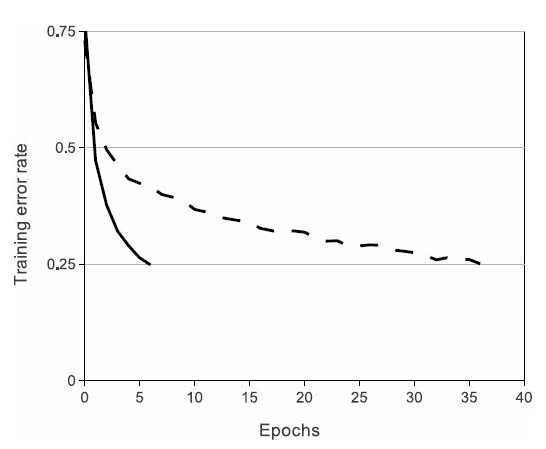
\includegraphics[width=0.5\textwidth]{figures/ReLU.jpg}
%\caption{Effect of using network with ReLUs (solid line) compared to a network with $tanh$ neurons (dashed lines)~\cite{krizhevsky2012imagenet}}
%\label{relu}
%\end{figure}

\subsection{The Unreasonable Effectiveness of Recurrent Neural Networks}
\par The CNNs used in the previous work~\cite{krizhevsky2012imagenet} is driven by prior understanding of how shape detection works. In ~\cite{karpathy2016unreasonable} the network design is based on prior information about the type of input which in this instance are sequences. Sequences are characterized as a time dependent function, which means that the entire input (output) is not available (formed) in a single instance. A nice example would be reading (input type) and writing (output type). Just as we have to know what we have read (written) so far in order to make sense of what we are going to read (write) next, the network architecture dealing with sequences is memory based with a feedback loop. If we recall, CNNs had the entire image at once over which the local receptive fields move.
\par Recurrent neural networks (RNNs) process sequences by maintaining a state variable which contains information of past inputs. Now that we have the building block the author suggests to \say{put on your deep learning hat and start stacking models up like pancakes}. Since the RNN model is very simple it does not capture long term dependencies very well. As error propagates back in time, the gradient vanishes by the time it reaches the initial steps~\cite{britz2015recurrent}. Hence, RNNs are not used in their vanilla state. The most popular variant are Long-Short Term Memory (LSTM) networks which use an elegant state preserving equation to control how much of information from the previous state should be used and how much information from the current state should be preserved~\cite{olah2015understanding}. The author of~\cite{karpathy2016unreasonable} uses character level inputs \emph{i.e.,} at time $t$ only one input neuron is active (corresponding to the input character) and the output is a distribution over the entire character set from which the character with the highest probability is the final output character which is again fed as input to generate the next character and so on. 
\par Let's checkmark the aspects we considered to be essential for deep learning. \textit{Non-linearity} - RNNs and its variants use neurons with non-linear output functions. \textit{Multi-layered representation} - the networks are layered and as illustrated in the visualization of RNNs in~\cite{karpathy2016unreasonable}, the author tries to interpret what the neurons may represent (recognizing \textit{URLs}, scopes, sentence endings and so on). None of these text structure recognition features are hand-crafted.

\subsection{Google's Deep Dream Images}
\par In~\cite{karpathy2016unreasonable}, the author presents a visualization of a trained text generating network by producing a heatmap of the neurons for each character input and out of the millions of neurons illustrates a few which is interpretable by humans. Similarly, we can look at visualizing any deep networks. The network considered in~\cite{tyka2015inceptionism} is an image classification deep CNN (similar to the network presented in~\cite{krizhevsky2012imagenet}) and the goal is to visualize the class models learned by the network. This is achieved by switching the direction of the connections - we start out with the class which we want to visualize and a noisy image (or zero image~\cite{simonyan2013deep}).The aim is to find that image $I$ which solves
\begin{equation}
argmax_{I} S_{c}(I) - \lambda \vert\vert I \vert\vert_{2}^{2}
\end{equation}
The image is formed by performing back-propagation through the network and instead of updating the network weights, the image is updated. The image formed is better when prior constraints like local continuity is imposed. Finally we get images which show us how the network represents a certain class - by its distinguishing color, shape or pattern. 
\par Now that we know how to generate an image from a trained classification network, what happens if we feed a regular image to the network, let the network classify it and ask the network to enhance the image using this class information or information from any lower levels? This gives the dream images described in~\cite{titcomb2016google}. As we move up the layers, the images get enhanced with distinguishing strokes or patterns or objects. The more the number of iterations the more vivid is the resulting image. 
\par The dream images are not a result of training a network from scratch but a means of understanding how an already trained network represents an image - what are the features in an image that it picks up which finally enable it to classify the image into a category. 

\subsection{Mastering the Game of GO with Deep Neural Networks and Tree Search}
\par In all the cases considered till now the deep networks operated in an environment where the output from the network did not affect the next input. The RNNs come close but, in the case we considered, the RNNs directly used the output as its next input. What we look at now is an interactive network which perceives an environment in a state and executes some actions which change the state of the environment. Based on the action and the effect on the environment the network is rewarded or penalized. The network takes into account this reward accumulated over time to train the network. This is what is termed as reinforcement learning~\cite{karpathy2016deep}. With the game of GO~\cite{silver2016mastering}, the authors develop a network which interacts with an environment which has a defined state space (a state is the orientation of the game pieces on the board) and a fixed set of actions.
\par The network uses multiple concepts to achieve its final winning rate of $99.8\%$ against other GO programs and to defeat human professional player. The network training includes a supervised learning of a dataset of 30 million GO moves. The network is then trained with reinforcement learning with rewards only in terminal steps to train the best policy, where the policy is basically a strategy to select the best move at a given state. A value network is trained using reinforcement learning to evaluate the outcome of the game from the current state using the policy from the policy network. The final program, AlphaGo follows a Monte Carlo Tree search algorithm for a lookahead search with the help of the trained policy and value networks to select actions.
\par Since the search space of GO is so vast (breadth wise and depth wise) simple tree search is infeasible. The concept of reinforcement learning is applied to a multi-layered network with the goal that the network learns some high-level representation of the game to judge which actions to take from just the state of the game. The multiple stages in the training is definitely not a purely deep learning process. There are manipulations of the network outcomes - like the using a lookahead search with the network outcomes to determine the best move is feature engineering, however, what kind of features the network learns in the intermediate layers to arrive at a decision is not hand-crafted.   

%\section{Is Deep Learning the Central Protagonist?}
\section{Is Deep Learning Actually Deep?}
\par From image recognition to sequence generation, network visualization to playing the game of GO, what unites all the approaches is the ability of a multi-layered network to represent abstraction from raw data available in large amounts. This is then guided by our prior knowledge regarding the field of application. For instance, using CNNs to interpret images or locally correlated structures, RNNs to generate sequences and reinforcement learning to interpret strategy games. For applications like image captioning both CNNs and RNNs are necessary. Hence, to answer the question - Is there a unified deep learning algorithm? - currently, the networks are very much dependent on our prior knowledge which makes the algorithms used in one field (computer vision) different from another (natural language processing).
\par We cannot manually control the network parameters individually (there are millions of parameters) and neither do we have enough understanding of what each neuron's function is or what triggers the neuron. We are bound to depend on error propagation to train the network. The network is also vulnerable to inherent bias in our training data which shows up as unexpected results - mostly good (things we've seen so far), sometimes bad~\cite{khurshudov2015suddenly} and sometimes, well ugly~\cite{curtis2015google}.
\par We want our networks to pick up representative features of the classes and that is what the networks do. So in~\cite{khurshudov2015suddenly} as pointed out by the author the leopard print is a very distinctive feature of the animal coupled with the facts that the training dataset may contain rare or no instance of a leopard print sofa and the variability in animal shapes due to postures and partial blocking, it is but understandable that a leopard print chair is classifies as a leopard. Similarly the case holds for the labeling in Google Photos~\cite{curtis2015google}. The classifier picks up the bias in the representation of human faces in the dataset. So, the nearest thing that matches a colored human head which in this case was gorilla is the final label of the classifier. These instances bring out the gap in human learning and AI learning which is still far from mimicking human learning.
\par Surely the argument presented in~\cite{khurshudov2015suddenly} about feeding thousands of data (original and transformed) does not mimic human learning is convincing. But, what we definitely did was tracing digits and alphabets and fill pages  learning the right curves to make the alphabets or digits all of which could be well qualified for an MNIST dataset. Getting a star from the teacher was the reinforcement leaning for our brain nets. It is kind of a chicken egg problem - unless we know how to drive a car, we cannot develop an autonomous car. In conclusion - is deep learning related to data mining or knowledge discovery? - maybe, it's just stacks of neuron layers waiting to be moulded into the right design architecture.  

\bibliographystyle{IEEEtran}
\bibliography{report1}
\end{document}